%!TEX root=../../main.tex
\section{Datenschnittstelle und Webseitenlogik}
\subsection{Webseitenlogik}
Wie in Kapitel \hyperref[sec:webseitenlogik]{6.3.1} beschrieben wird die Webseitenlogik größtenteils von einem Manager übernommen.

\subsubsection{Navigation}
\label{sec:navigation}
Die Unterseiten werden in den Manager geladen und je nach Gebrauch angezeigt. Dafür gibt es eine Variable im Manager, welche dafür sorgt, dass nur eine Komponente auf einmal angezeigt werden kann. Die Komponente wird gewechselt, indem die nachfolgende Funktion aufgerufen wird:
\begin{code}{js}
	changeComponent(
	component,
	back = true,
	application = null,
	escortsdata = null
	) {
		switch (component) {
			case "Login":
			this.change("Login", back);
			this.deleteCookie();
			break;
			
			case "Index":
			this.change("Index", back);
			break;
			
			case "ApplicationView":
			this.loadApplication(application);
			this.change("ApplicationView", back);
			break;
			
			case "Escorts":
			this.loadEscortsData(escortsdata);
			this.change("Escorts", back, false);
			break;
			
			// [Weitere Unterseiten]
		}
	}
\end{code}
\captionof{listing}{Funktion zum ändern der angezeigten Komponente}~\\
\newpage
Diese Funktion besteht hauptsächlich aus einer Verzweigung, welche Seite angezeigt werden soll.
Des weiteren gibt es bei manchen Komponenten den Zusatz einer load Funktion, welche Daten für die jeweilige Komponente vorbereitet bzw. berechnet.

Die referenzierte \textit{change} Funktion übernimmt das tatsächliche ändern der Variable:
\begin{code}{js}
	change(page, back = true, cookie = true) {
		this.currentComponent = page;	// Es wird die angezeigte Seite verändert
		window.scrollTo(0, 0);	// Es wird zum Anfang der Seite gegangen
		if (back) {
			if (window.history.state !== page) {
				window.history.pushState(page, null);	// Es wird die übergebene Seite in die History des Browsers geschrieben
			}
		}
		if (cookie) {
			this.setCookie(page);	// Es wird der Cookie gesetzt
		}
\end{code}
\captionof{listing}{Funktion für das Managment der Cookies und History des Browsers}~\\
Hier wird nicht nur die angezeigte Seite verändert, sondern auch die Cookies, sowie die History des Browsers gesetzt. Es wird je nach Parameter der Cookie und die History gesetzt.\\
Die beschriebenen Funktionen müssen von den Komponenten aufgerufen werden können, deswegen hört der Manager auf Signale der Unterseiten, falls diese die Seite ändern möchte. Dies wird mittels VueJS erledigt, da das Framework dafür bereits Funktionen implementiert hat:
\begin{code}{js}
	v-on:change-component="changeComponent"
	// Es wird auf das Signal change-component gehört und die Funktion changeComponent aufgerufen
\end{code}
\captionof{listing}{Event Handling mittels v-on}~\\
Die Codezeile wird beim Aufruf der Unterseite im Manager hinzugefügt.\\
Die beschriebenen Signale werden von den Unterseiten mittels folgendem Code bzw. Funktion gesendet:
\begin{code}{js}
	changeComponent(component, back, application, escortsdata) {
		this.\$emit("change-component", component, back, application, escortsdata);
	}
\end{code}
\captionof{listing}{Signal senden}~\\
Hier wird durch \textit{this.\$emit()} ein Befehl an die übergeordnete Seite gesendet.
\newpage
\subsubsection{Komponenten}
Die Komponenten der Unterseiten werden, wie im vorherigen Kapitel beschrieben, in den Manager eingebunden. Dies wird mit dem Import, Laden und Implementierung der Komponente umgesetzt.
Das Importieren erfolgt mit folgendem Code:
\begin{code}{html}
	<script>
	import ApplicationView from "@/components/ApplicationView.vue";
	// [Weitere Imports]
	
	export default {
		components: {
			ApplicationView
			// [Weitere Komponenten]
		}
	}
</script>
\end{code}
\captionof{listing}{Importieren und Laden einer Komponente}~\\
In dem Code wird von \textit{@/components/} die einzelnen Komponenten geladen. Aufgrund der Verwendung von @ wird das Angeben des vollen Pfades nicht mehr gebraucht, da dies auf den relativen Pfad der Softwarestruktur zeigt.
\newpage
Diese Komponente muss noch in den Manager angezeigt werden. Dies wird in dem Template des Managers mit folgendem Code umgesetzt:
\begin{code}{html}
<template>
	<div class="home">
		<Login
			v-if="currentComponent == 'Login'"
			v-on:change-component="changeComponent"
			v-bind:url="url"
			v-bind:token="token"
			v-bind:forward="forward"
			v-on:requestAnswer="useCookie"
			v-bind:cookieset="cookies"
			v-on:login="login"
		/>
		<Index
			v-if="currentComponent == 'Index'"
			v-on:change-component="changeComponent"
			v-bind:url="url"
			v-bind:token="token"
			v-bind:admin="admin"
			v-bind:user="user"
		/>
		<ApplicationView
			v-if="currentComponent == 'ApplicationView'"
			v-on:change-component="changeComponent"
			v-bind:url="url"
			v-bind:token="token"
			v-bind:appid="appid"
			v-bind:user="user"
		/>
		<PageNotFound
			v-if="currentComponent == 'PageNotFound'"
			v-on:change-component="changeComponent"
			v-bind:url="url"
		/>
		<!-- Weitere Komponenten -->
	</div>
</template>
\end{code}
\captionof{listing}{Anzeigen der Komponenten im Manager}~\\
In dem Code wird nicht nur die Komponente angezeigt, sondern auch Daten an die Komponenten gebunden.\\
\textit{v-if} Attribute sorgen dafür, dass das Rendern nur unter der angegebenen Bedingung erfolgt. In dem Fall wird die Komponente nur angezeigt, wenn die Variable currentComponent den Namen einer Komponente annimmt.\\
\textit{v-bind} Attribute binden Daten von der übergeordneten Komponente in die eingebundene Komponente. Bei dem Beispiel \textit{v-bind:cookieset=''cookies''} wird an die Login-Komponente ein Attribut cookieset mitgegeben mit dem Wert von der Variable cookies.
\newpage
Diese Attribute können mit folgendem Code aufgefangen werden und in diesen eingebundenen Komponenten verwendet werden:
\begin{code}{html}
		props: ["url", "forward", "cookieset"]
\end{code}
\captionof{listing}{Auffangen einer übergebenen Variable}~\\
In dem Code werden die übergebenen Variablen, welche in der übergeordneten Komponente definiert worden sind, aufgefangen. Diese können als normale Variable verwendet werden.
\newpage
\subsubsection{Seite nicht gefunden}
Wie in Kapitel \hyperref[sec:not_found]{6.3.1.1} beschrieben wird, wird der Benutzer bei Eingabe eines falschen Links auf eine Seite weitergeleitet. Dazu wird der Vue-Router so eingestellt, sodass jeder Link, außer der Hauptlink zur eigentlichen Webseite, auf die beschriebene Seite weitergeleitet wird. Die Routen des Routers sind wie folgt aufgebaut:
\begin{code}{js}
// Imports für die Komponenten
import Vue from "vue";
import VueRouter from "vue-router";
import Home from "../views/Home.vue";
import PageNotFound from "../components/PageNotFound.vue";

Vue.use(VueRouter);		// Sagt dem Projekt, dass es den Router verwenden soll

const routes = [
{
	path: "/",					// Der Pfad, der von dem Benutzer eingegeben wird
	name: "Home",				// Der Name des Pfades
	component: Home,			// Die Komponente, welche angezeigt werden soll
	props: { pathing: "base" }	// Variablen, welche an die Komponente gesendet werden sollen
},
{
	path: "/viewer",
	name: "Viewer",
	component: Home,
	props: route => ({ query: route.query.uuid })	// Die ID des Antrags, welcher betrachtet werden möchte
},
{
	path: "*",				// Fasst alle nicht erwähnten Routen zusammen
	name: "NotFound",
	component: PageNotFound
}
];
const router = new VueRouter({
	mode: "history",
	base: process.env.BASE_URL,
	routes
});

export default router;
\end{code}
\captionof{listing}{Router, welcher die Pfade der Software verwaltet}~\\

Wird ein Link eingegeben, welcher nicht ''/'' oder ''/viewer'' entspricht, so wird die \textit{PageNotFound} Komponente geladen und dem Benutzer mitgeteilt, dass der eingegebene Link nicht funktioniert.
\subsubsection{Antrag-Viewer}
\label{sec:antrag_viewer}
Der Antrag-Viewer wird über den Link \textit{/viewer} aufgerufen. Dies führt dazu, dass der Benutzer auf eine Seite weitergeleitet wird, auf der er die ID eines Antrags eingeben kann.
\begin{figure}[H]
	\centering
	
\includegraphics[width=1\linewidth]{images/antrag_viewer}
	\caption[Webseite Antrag-Viewer]{Die Antrag-Viewer Seite der Webseite}
	\label{fig:antragviewer}
\end{figure}

Sollte der Benutzer nicht angemeldet sein, so wird er zuerst auf die Login-Seite weitergeleitet, bevor er die ID des Antrags eingeben kann. Sollte der eingegebene Link bereits den Parameter \textit{uuid} besitzen, wird der Benutzer auf die Antragsansichtsseite weitergeleitet, sofern dieser angemeldet ist. Ansonsten wird der Benutzer zuerst auf die Login-Seite weitergeleitet.
\begin{code}{js}
	{
		// Die Route des Antrag-Viewers
		path: "/viewer",
		name: "Viewer",
		component: Home,
		props: route => ({ query: route.query.uuid }) // Der Parameter in der URL
	},
\end{code}
\captionof{listing}{Route für den Antrag-Viewer}~\\
Es wird die Home-Komponente (der Manager) aufgerufen, da dieser das Verarbeiten der URL und das Weiterleiten auf die Login und Antragsansicht übernimmt.
\newpage
\subsubsection{Features}
Die in Kapitel \hyperref[sec:feature]{6.3.1.6} Features wurden folgendermaßen implementiert.

\paragraph{Zuletzt besuchte Seite der Webseite}~\\
Beim Laden der Webseite wird mithilfe von Cookies auf die zuletzt besuchte Seite navigiert. Dazu wird bei jeder Navigation, wie in Kapitel \hyperref[sec:navigation]{7.1.1.1} beschrieben, der Cookie gesetzt. Dieser wird beim Laden der Webseite aufgerufen und es wird, falls der Cookie gesetzt ist, auf diese Seite navigiert.
\begin{code}{js}
	if (this.checkCookie()) {		// Abfrage, ob ein Cookie vorhanden ist
		this.useCookie(true);		// Sofern ein Cookie vorhanden ist, hat der Benutzer bereits die Cookies für diese Webseite akzeptiert
		var c = this.getCookie();	// Die Informationen des Cookies werden ausgelesen
		if (c == this.generateState(window.history.state)) {	// Falls die zuletzt besuchte Seite die gleiche ist, wie die aktuelle Seite, so wird kein neuer Eintrag in der History generiert
			this.changeComponent(c, false);
		} else {
			this.changeComponent(c);
		}
	} else {
		// Falls kein Cookie gesetzt ist, wird der Benutzer auf die Login-Seite weitergeleitet
		this.changeComponent("Login");
	}
\end{code}
\captionof{listing}{Navigation auf die zuletzt besuchte Unterseite}~\\

\paragraph{Browser-Pfeile}~\\
Die Browser-Pfeile navigieren durch die History des Browsers. Da die Webseite ein One-Pager ist, muss das Schreiben in die History selbst übernommen werden. Dies wird durch den folgenden Code umgesetzt:
\begin{code}{js}
window.addEventListener("popstate", e => {			// Es wird ein Listener auf die Webseite gesetzt
	if (this.generateState(e.state) === "Escorts") {	// Dies ist eine extra Abfrage, welche verhindert auf die Escorts-Seite zu gelangen.
		this.changeComponent("School", false);
	} else {
		this.changeComponent(this.generateState(e.state), false);	// Es wird auf die Unterseite navigiert.
	}
});
\end{code}
\captionof{listing}{Unterstützung der Browser-Pfeile}~\\
Das Hinzufügen der einzelnen Histories für die einzelnen Unterseiten wird in Kapitel \hyperref[sec:navigation]{7.1.1.1} beschrieben.
\newpage
\subsection{Anmelden}
Der Benutzer kann sich auf einer Anmelde-Seite anmelden um das System verwenden zu können. Dazu werden die Anmeldedaten des Benutzers an das Backend gesendet. Um sich anmelden zu können, müssen die Cookies akzeptiert werden. Sollten jene nicht akzeptiert werden, ist es nicht möglich den Dienst zu verwenden.
Sobald der Benutzer erfolgreich angemeldet ist, wird dieser auf die Hauptseite weitergeleitet.
\\
\begin{code}{js}
axios.post(this.url + "/login", {	// Sendet ein POST-Abfrage an das Backend
	username: this.email,	// Die eingegebene E-Mail Adresse
	password: this.password // Das eingegebene Passwort
}).then(response => {
	var data = response.data
	// Es werden die Daten aus der Abfrage an den Manager gesendet, damit eine valide Sitzung erstellt wird.
})
\end{code}
\captionof{listing}{POST-Abfrage für den Login}~\\

\subsubsection{Spezielle Situationen}
In besonderen Fällen, wie in Kapitel \hyperref[sec:antrag_viewer]{7.2.1.4} beschrieben, wird der Benutzer nicht auf die Hauptseite weitergeleitet, sondern auf den Antrag-Viewer oder auf die Antrag Ansicht.
\begin{code}{js}
switch (this.forward.name) {	// Es wird entschieden, auf welche Unterseite navigiert werden soll
	case "ApplicationSearch":	// Es wird auf den Antrag-Viewer navigiert
	this.\$emit("change-component", this.forward.name);
	break;
	case "ApplicationView":	// Es wird auf die Antrag Ansicht navigiert
	this.\$emit(
	"change-component",
	this.forward.name,
	true,
	this.forward.id
	);
	break;
	default:	// Es wird auf die Hauptseite navigiert
	this.\$emit("change-component", "Index");
	break;
}
\end{code}
\captionof{listing}{Weiterleitung nach erfolgreichem Anmelden}~\\
\subsubsection{Passwort vergessen}
Da Refundable die Anmeldedaten von LDAP-verwendet, wird, wenn auf ''Passwort vergessen'' gedrückt wird, der Benutzer auf \href{https://owa.tgm.ac.at}{OWA} weitergeleitet.
\newpage
\subsection{Abmelden}
Wird auf den ''Abmelden'' Knopf gedrückt, wird ein Abfrage mit dem derzeit aktiven Token an das Backend gesendet, um den Authentifizierungstoken zu terminieren. Dies bedeutet, dass der Benutzer keinen validen Token mehr besitzt und auf die Login Seite weitergeleitet wird.
\begin{code}{js}
axios.post(this.url + "/logout", {	// Sendet ein POST-Abfrage an das Backend
	headers: { Authorization: this.token }	// Der Token des Benutzers
})
.then(response => {
	if (response.status === 200) {	// Falls die Abfrage erfolgreich war
		this.token = "";
		this.refresh_token = "";
		this.deleteCookie();
		this.changeComponent("Login");	// Es werden die Tokens und Cookies gelöscht und der Benutzer wird auf die Login-Seite weitergeleitet.
	}
});
\end{code}
\captionof{listing}{Gesamte Abfrage für das Abmelden}~\\
\newpage
\subsection{Antrag erstellen}
Ein Antrag kann von jedem Lehrer, der an dem System angemeldet ist, erstellt werden. Dazu wird auf die Antrag erstellen Unterseite navigiert, wo der Benutzer aussuchen kann, ob er eine Schulveranstaltung, Fortbildung oder einen anderen Antrag erstellen möchte. Auf diesen Unterseiten werden die notwendigen Informationen von dem Benutzer in die Eingabefelder eingegeben. Diese Informationen werden in ein JSON-Objekt gegeben und an das Backend gesendet.
\\
In den folgenden Codebeispielen, werden oft die Befehle \textit{returnString}, \textit{returnBoolean} und \textit{returnValue} verwendet. Diese dienen dazu die Datentypen auf die des Backends anzupassen. 
\subsubsection{Schulveranstaltung}
\paragraph{Allgemeine Informationen}~\\
In dem ersten Schritt, werden allgemeine Informationen der Schulveranstaltung eingegeben.
\begin{figure}[H]
	\centering
	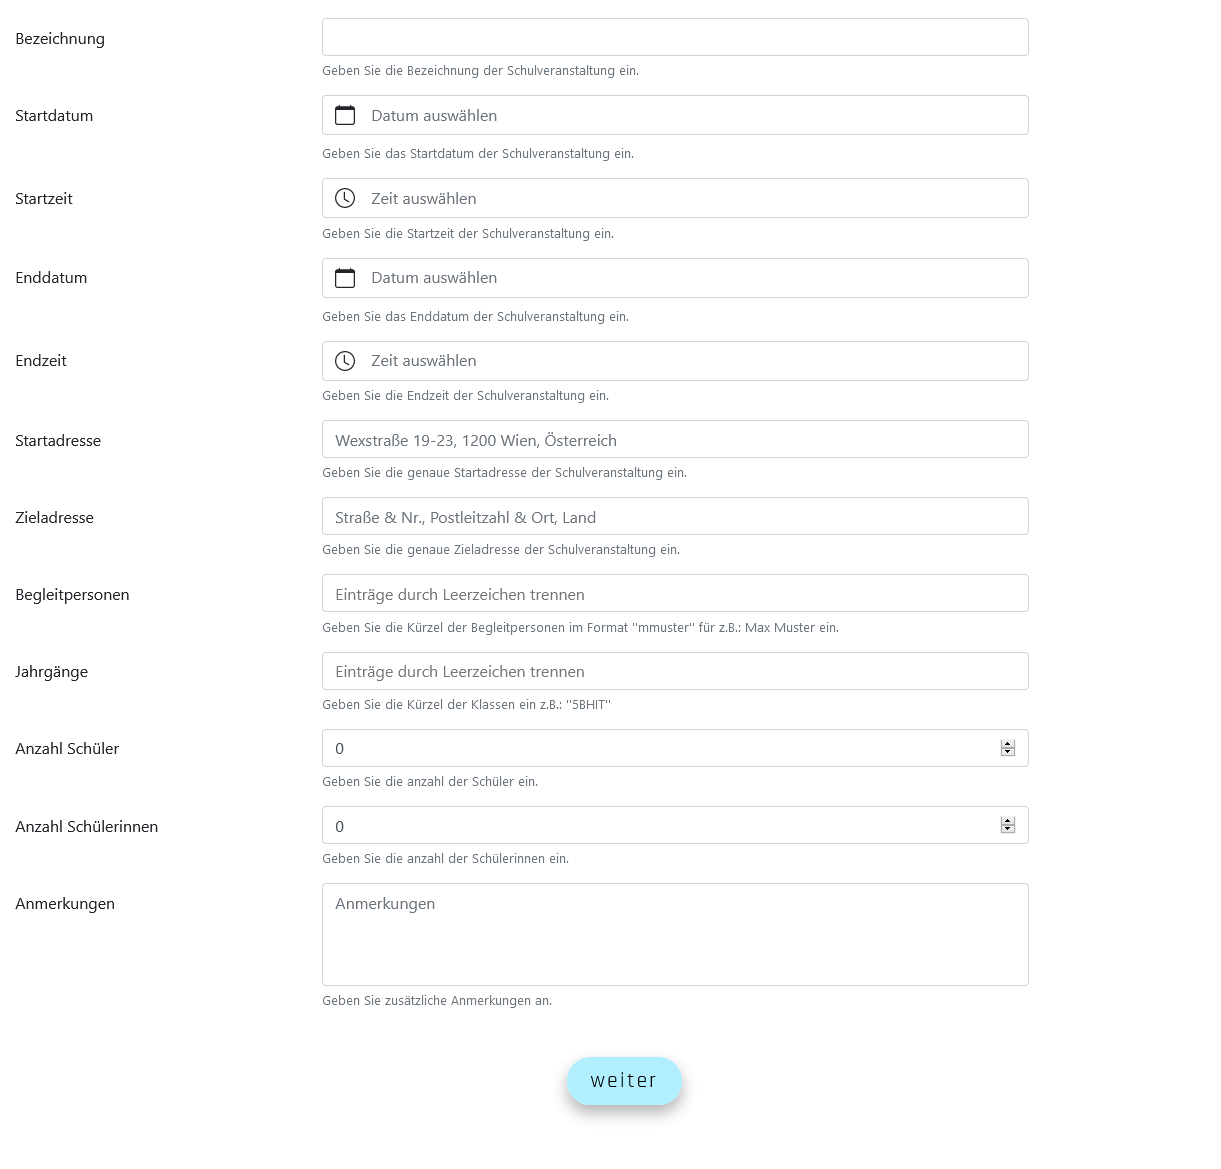
\includegraphics[width=1\linewidth]{images/schoolgeneral}
	\caption[Schulveranstaltung]{Eingabefelder für allgemeine Informationen einer Schulveranstaltung}
	\label{fig:schoolgeneral}
\end{figure}
\paragraph{Informationen zu Begleitlehrern}~\\
Nach der Eingabe aller allgemeinen Informationen wird der Benutzer nach dem Drücken des ''weiter'' Knopfes auf eine weitere Unterseite weitergeleitet. Auf dieser können Informationen zu den im vorherigen Schritt angegeben Begleitlehrern angegeben werden.
\begin{figure}[H]
	\centering
	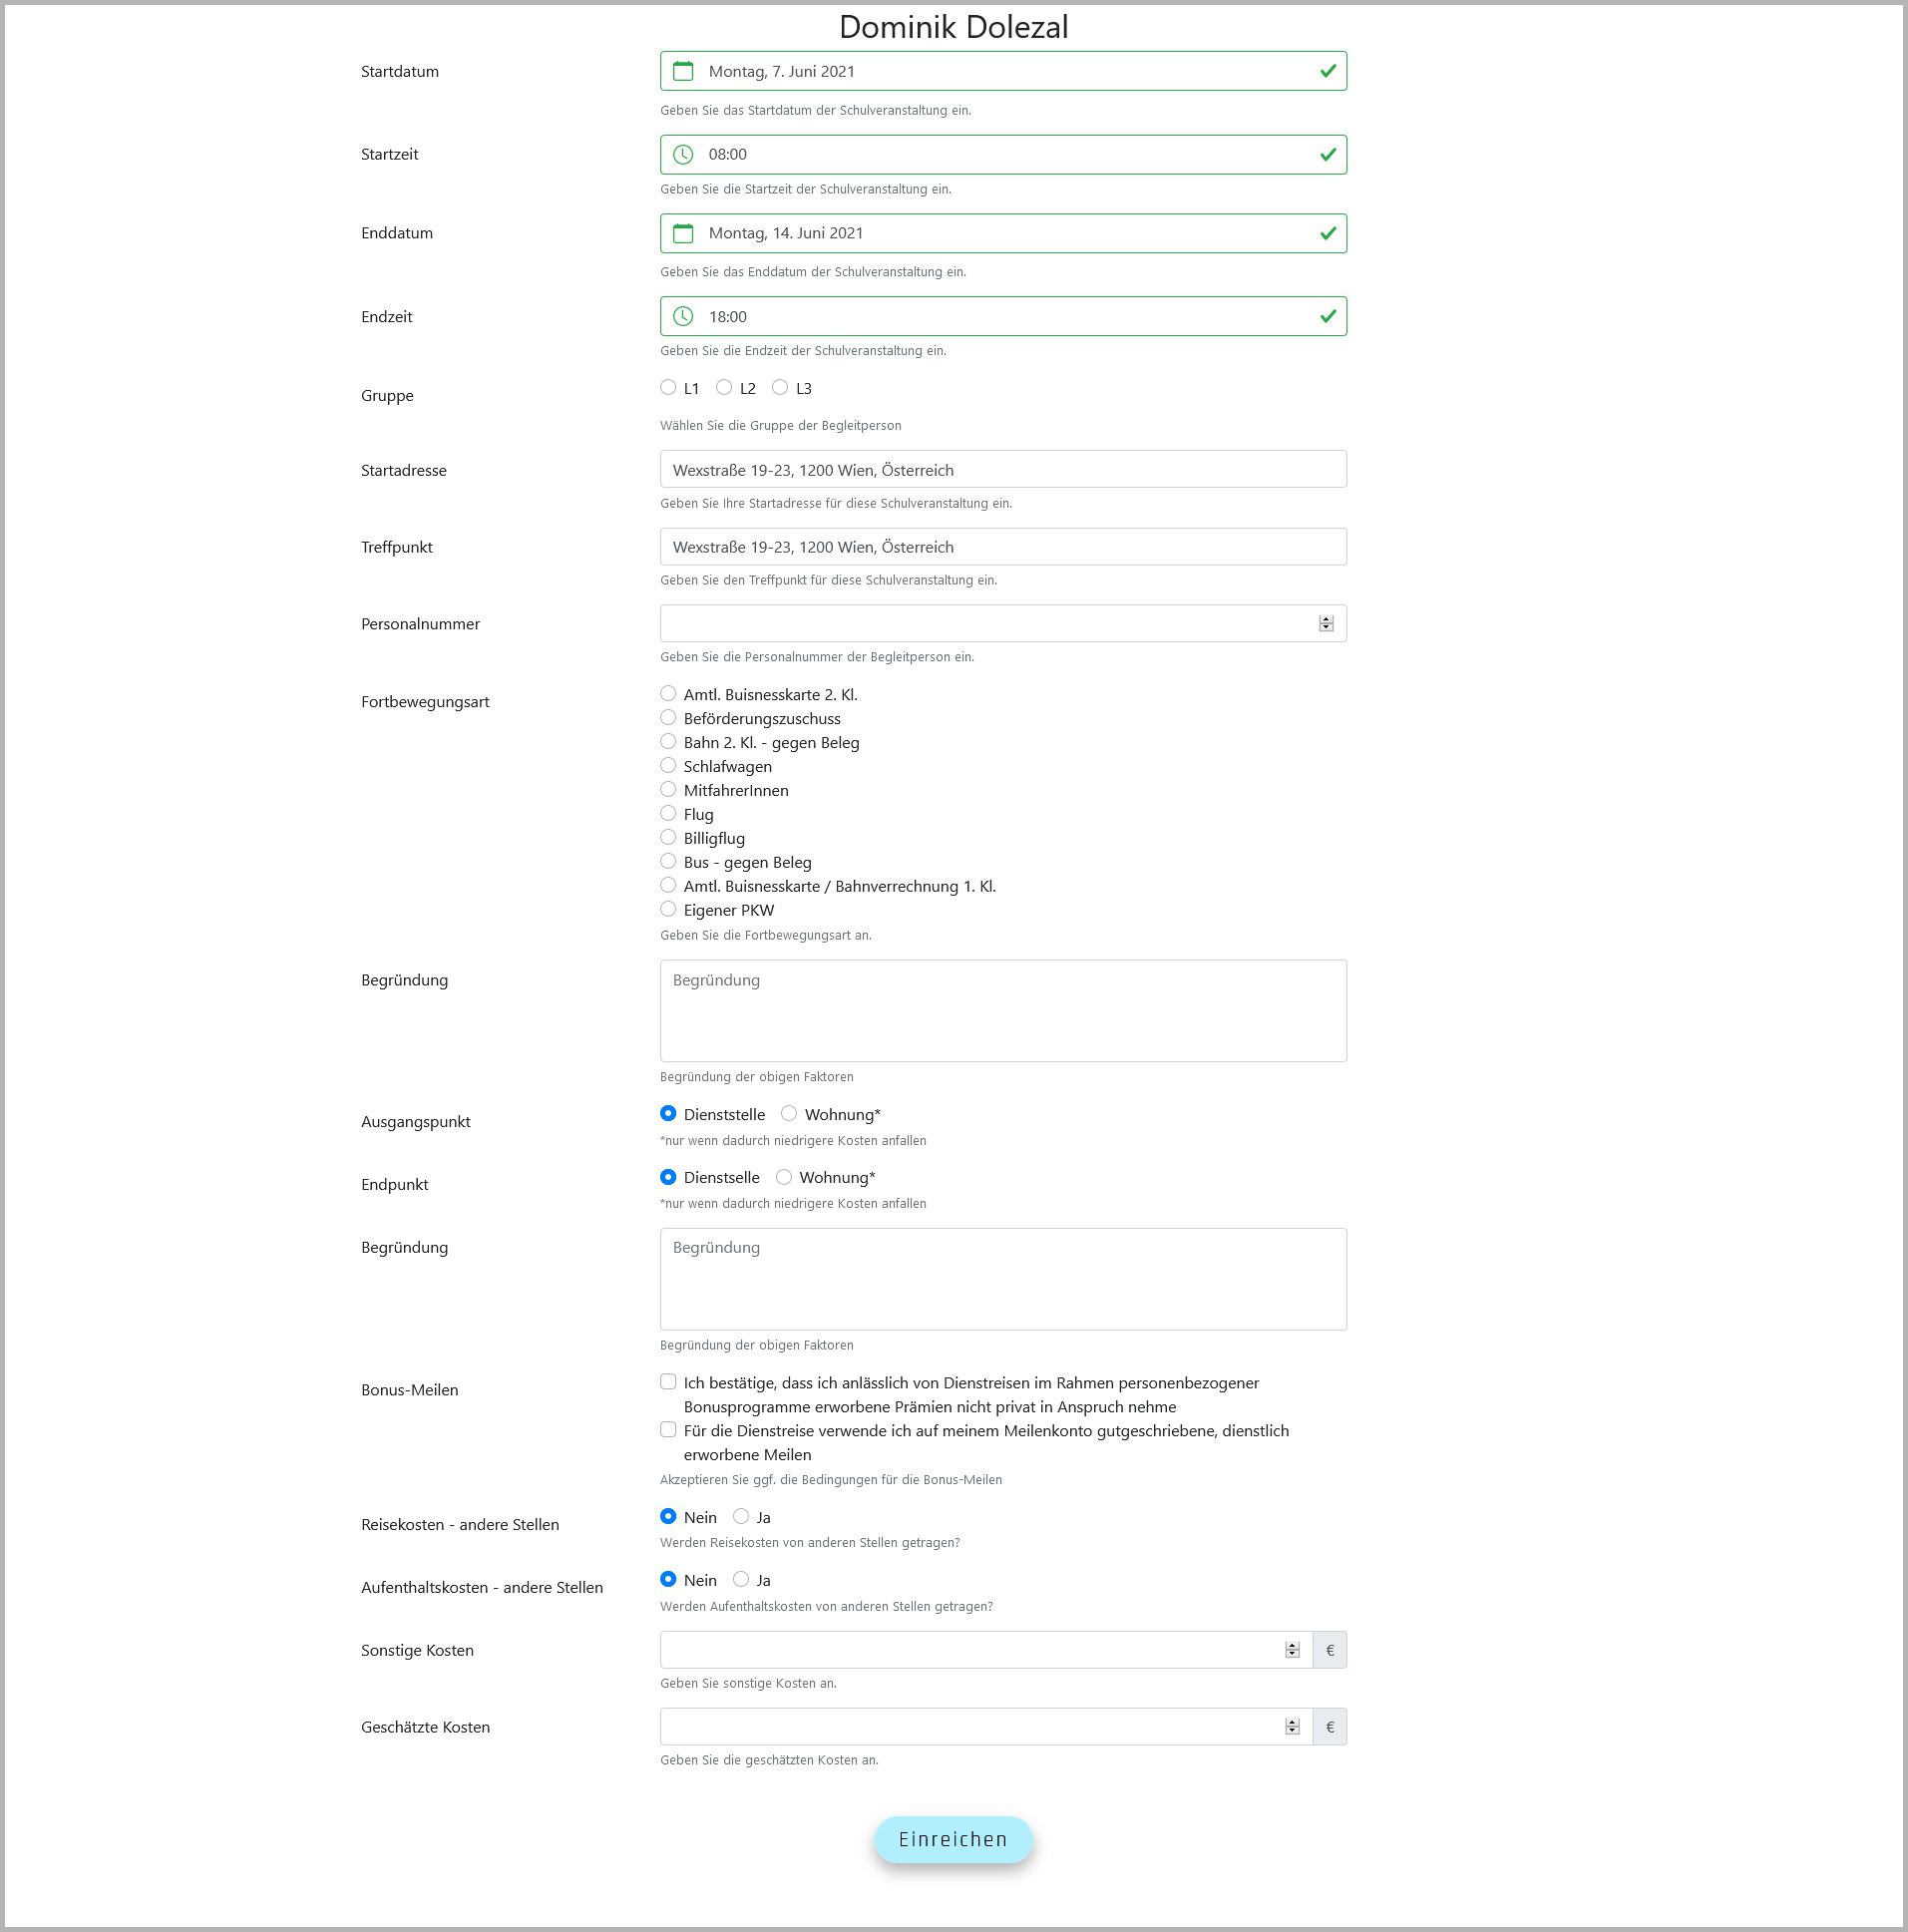
\includegraphics[width=1\linewidth]{images/escorts}
	\caption[Schulveranstaltung 2]{Eingabefelder für Informationen von Begleitlehrern}
	\label{fig:escorts}
\end{figure}
\newpage
Nachdem die Seite bearbeitet worden ist, kann auf den Knopf ''Einreichen'' gedrückt werden. Sobald der Knopf gedrückt worden ist, wird das JSON-Objekt, mit allen Informationen, die eingegeben worden sind, erstellt und an das Backend gesendet.
\label{code_submit_data}
\begin{code}{js}
var data = {		// Das JSON-Objekt mit allen Informationen
	Name: this.returnString(this.escorts.description),	// Der Name des Antrags
	Kind: 4,	// Der Typ des Antrags (4 = Schulveranstaltung)
	MiscellaneousReason: this.returnString(""),			// Nicht benötigt, da es eine Schulveranstaltung ist
	Progress: 1,	// Der Fortschritt ist standardmäßig auf 1 gesetzt
	StartTime: this.setTimezone(	// Die Startzeit des Antrags
	new Date(this.escorts.startDate + "T" + this.escorts.startTime)
	),
	EndTime: this.setTimezone(	// Die Endzeit des Antrags
	new Date(this.escorts.endDate + "T" + this.escorts.endTime)
	),
	Notes: this.returnString(this.escorts.notes),	// Zusätzliche Notizen zum Antrags
	StartAddress: this.returnString(this.escorts.start),	// Startadresse des Antrags
	DestinationAddress: this.returnString(this.escorts.ziel), // Zieladresse des Antrags
	SchoolEventDetails: {	// Allgemeine Informationen zu einer Schulveranstaltung
		Classes: this.escorts.class,	// Klassen, die auf die Schulveranstaltung mitfahren
		AmountMaleStudent: this.returnValue(	// Anzahl der männlichen Schüler der Schulveranstaltung
		this.escorts.count_student_male
		),
		AmountFemaleStudent: this.returnValue(	// Anzahl der weiblichen Schüler der Schulveranstaltung
		this.escorts.count_student_female
		),
		DurationInDays: this.returnValue(this.escorts.exkursLength),	// Die Länge der Schulveranstaltung in Tagen
		Teachers: teachers	// Eine Liste aller Lehrer mit Ihren spezifischen Informationen
	},
	BusinessTripApplications: business,	// Die Reiseformulare für alle Lehrer beteiligt an dem Antrag
	TravelInvoices: invoices	// Die Reiserechnungen für alle Lehrer beteiligt an dem Antrag
};
\end{code}
\captionof{listing}{JSON-Objekt einer Schulveranstaltung}~\\
\newpage
\subsubsection{Fortbildung}
Eine Fortbildung wird auf der Fortbildungs-Unterseite erstellt. Diese sieht wie folgt aus und beinhaltet Eingabefelder für alle notwendigen Informationen der Fortbildung.
\begin{figure}[H]
	\centering
	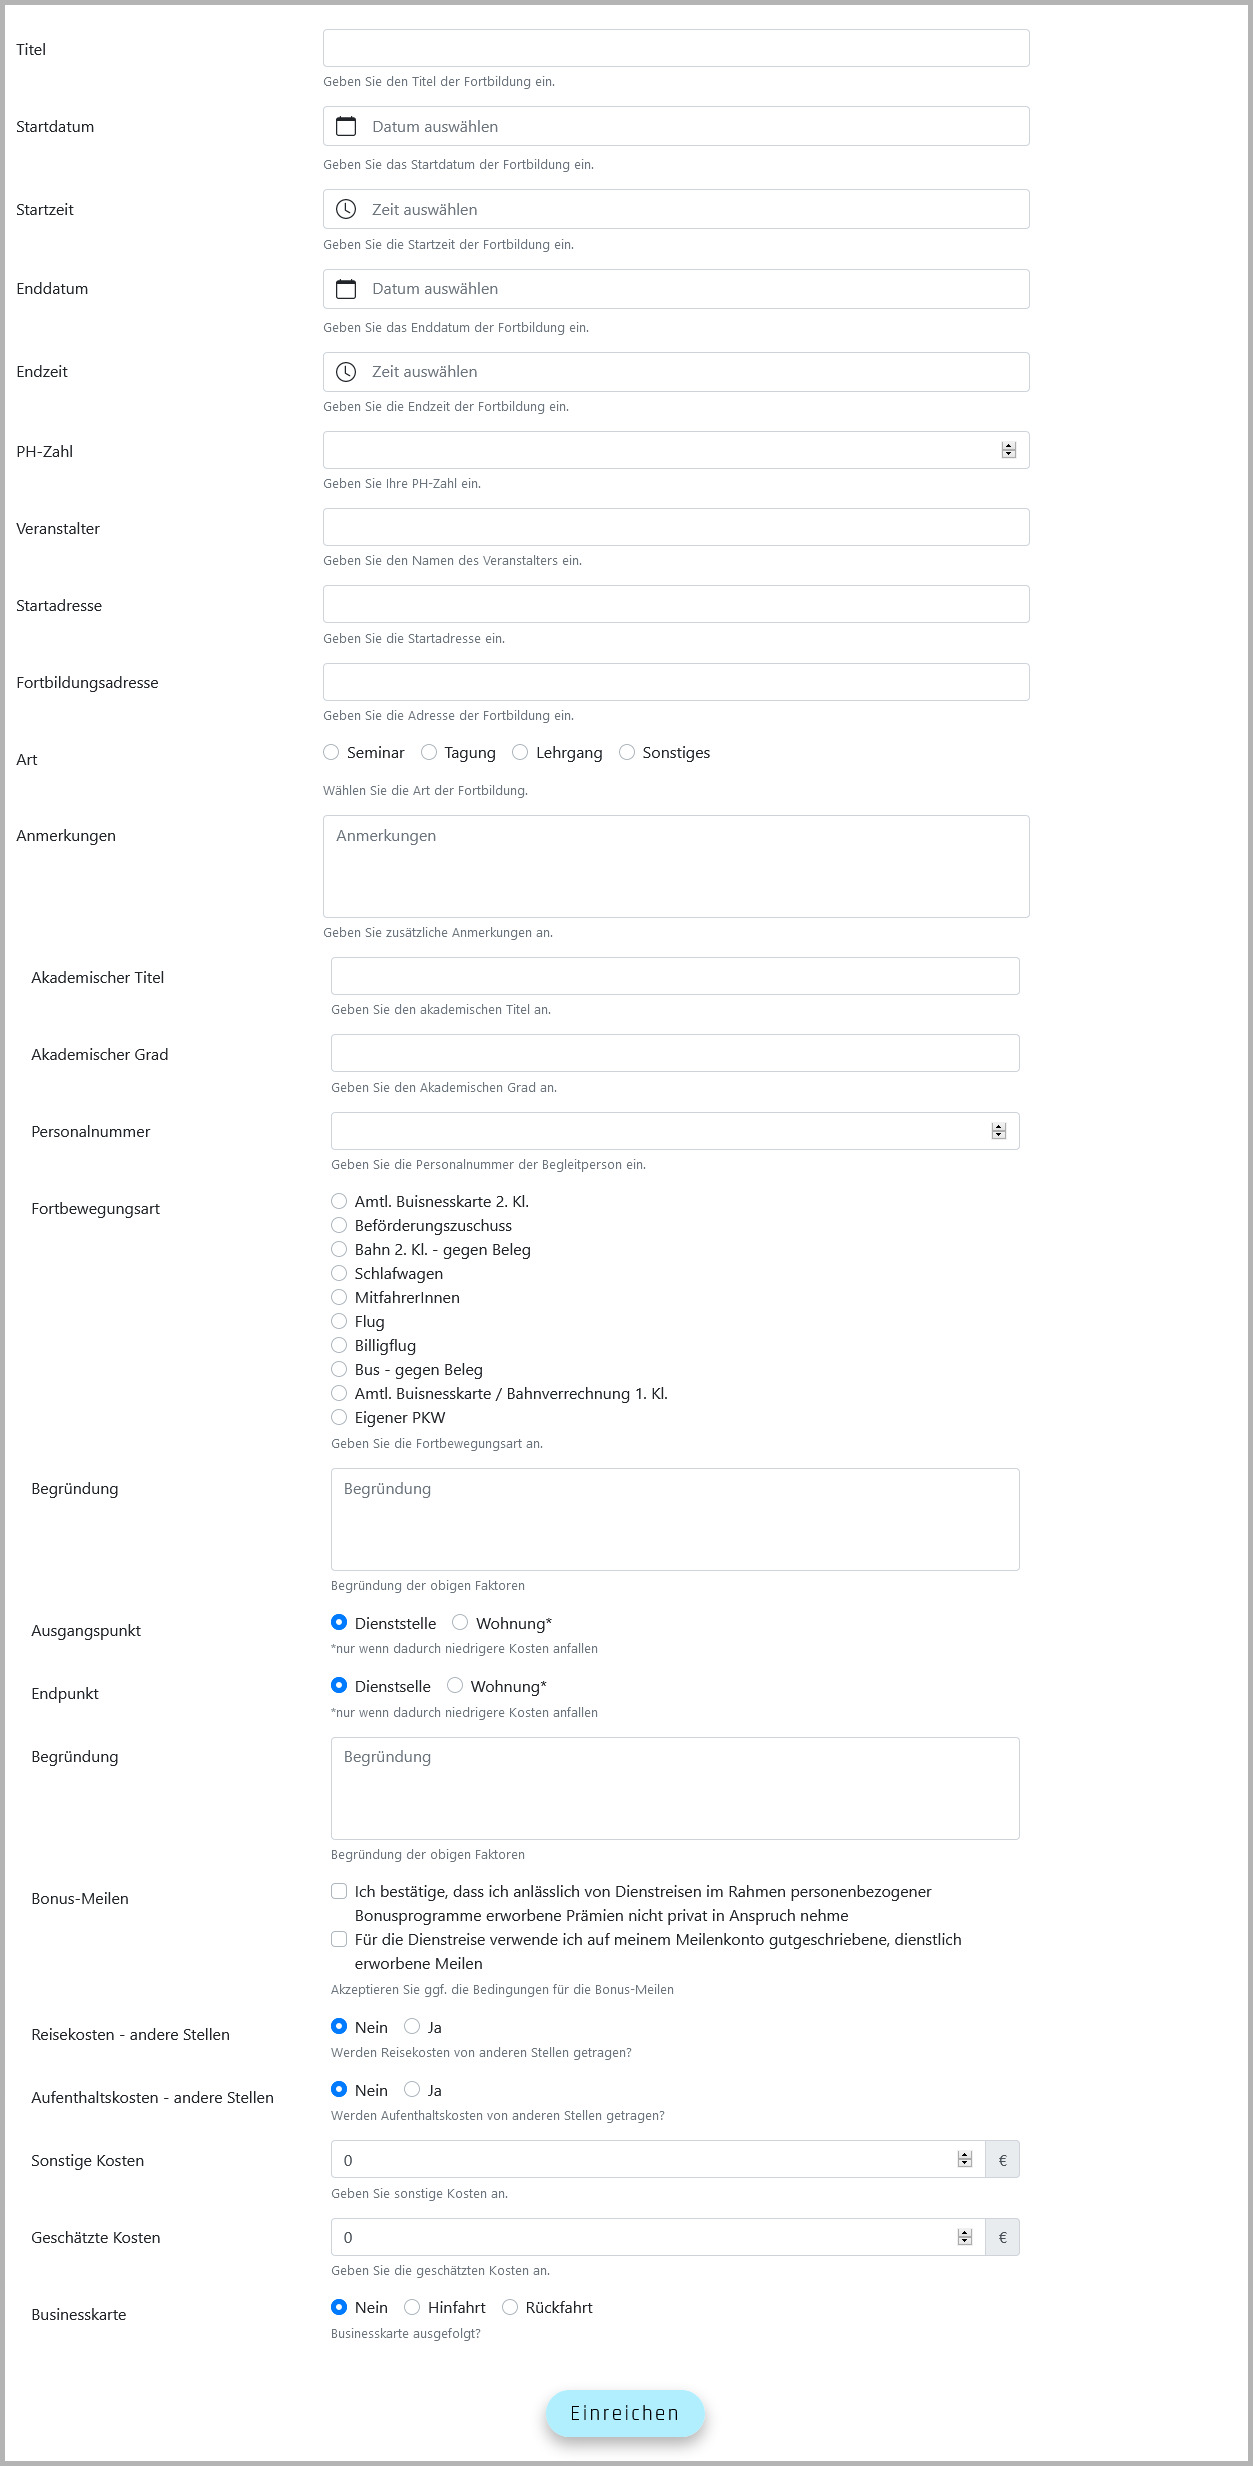
\includegraphics[width=0.65\linewidth]{images/workshop}
	\caption[Fortbildung]{Eingabefelder einer Fortbildung}
	\label{fig:workshop}
\end{figure}
\newpage
Bei einer Fortbildung kann unterschieden werden, welche Art von Fortbildung erstellt werden soll. Es kann zwischen Seminar, Tagung, Lehrgang und Sonstiges unterschieden werden. Das JSON-Objekt wird nach dem Drücken des ''Einreichen'' Knopfes erstellt und mit den angegebenen Daten befüllt. Das Objekt wird anschließend an das Backend gesendet.\\

Das JSON-Objekt wird, wie in Kapitel \hyperref[code_submit_data]{7.2.4.1} beschrieben, erstellt. Für eine Fortbildung gibt es nur wenige Änderungen.
Statt dem \textit{SchoolEventDetails} Objekt, wird ein \textit{TrainingDetails} Objekt in den Antrag hinzugefügt und die Art des Antrags wird auf 0 gesetzt:
\begin{code}{js}
var data = {		// Das JSON-Objekt mit allen Informationen
	Name: this.returnString(this.escorts.description),	// Der Name des Antrags
	Kind: 0,	// Der Typ des Antrags (0 = Fortbildung)
	// ...
	TrainingDetails: {
		Kind: this.returnValue(this.selected),	// Die Art der Fortbildung
		MiscellaneousReason: this.returnString(this.son),	// Falls "Sonstiges" ausgewählt worden ist
		PH: this.returnValue(this.phNumber),	// Die PH Zahl des Lehrers
		Organizer: this.returnString(this.veran)	// Der Veranstalter der Fortbildung
	},
	BusinessTripApplications: business,	// Das Reiseformular für den Lehrer
	TravelInvoices: invoices	// Die Reiserechnung für den Lehrer
};
\end{code}
\captionof{listing}{JSON-Objekt einer Fortbildung}~\\
\newpage
\subsubsection{Sonstiges}
Ein Sonstiger Antrag kann auf der Unterseite ''Anderer Grund'' erstellt werden. Ein Sonstiger Antrag sieht wie folgt aus und beinhaltet Eingabefelder für alle notwendigen Informationen für den Antrag.
\begin{figure}[H]
	\centering
	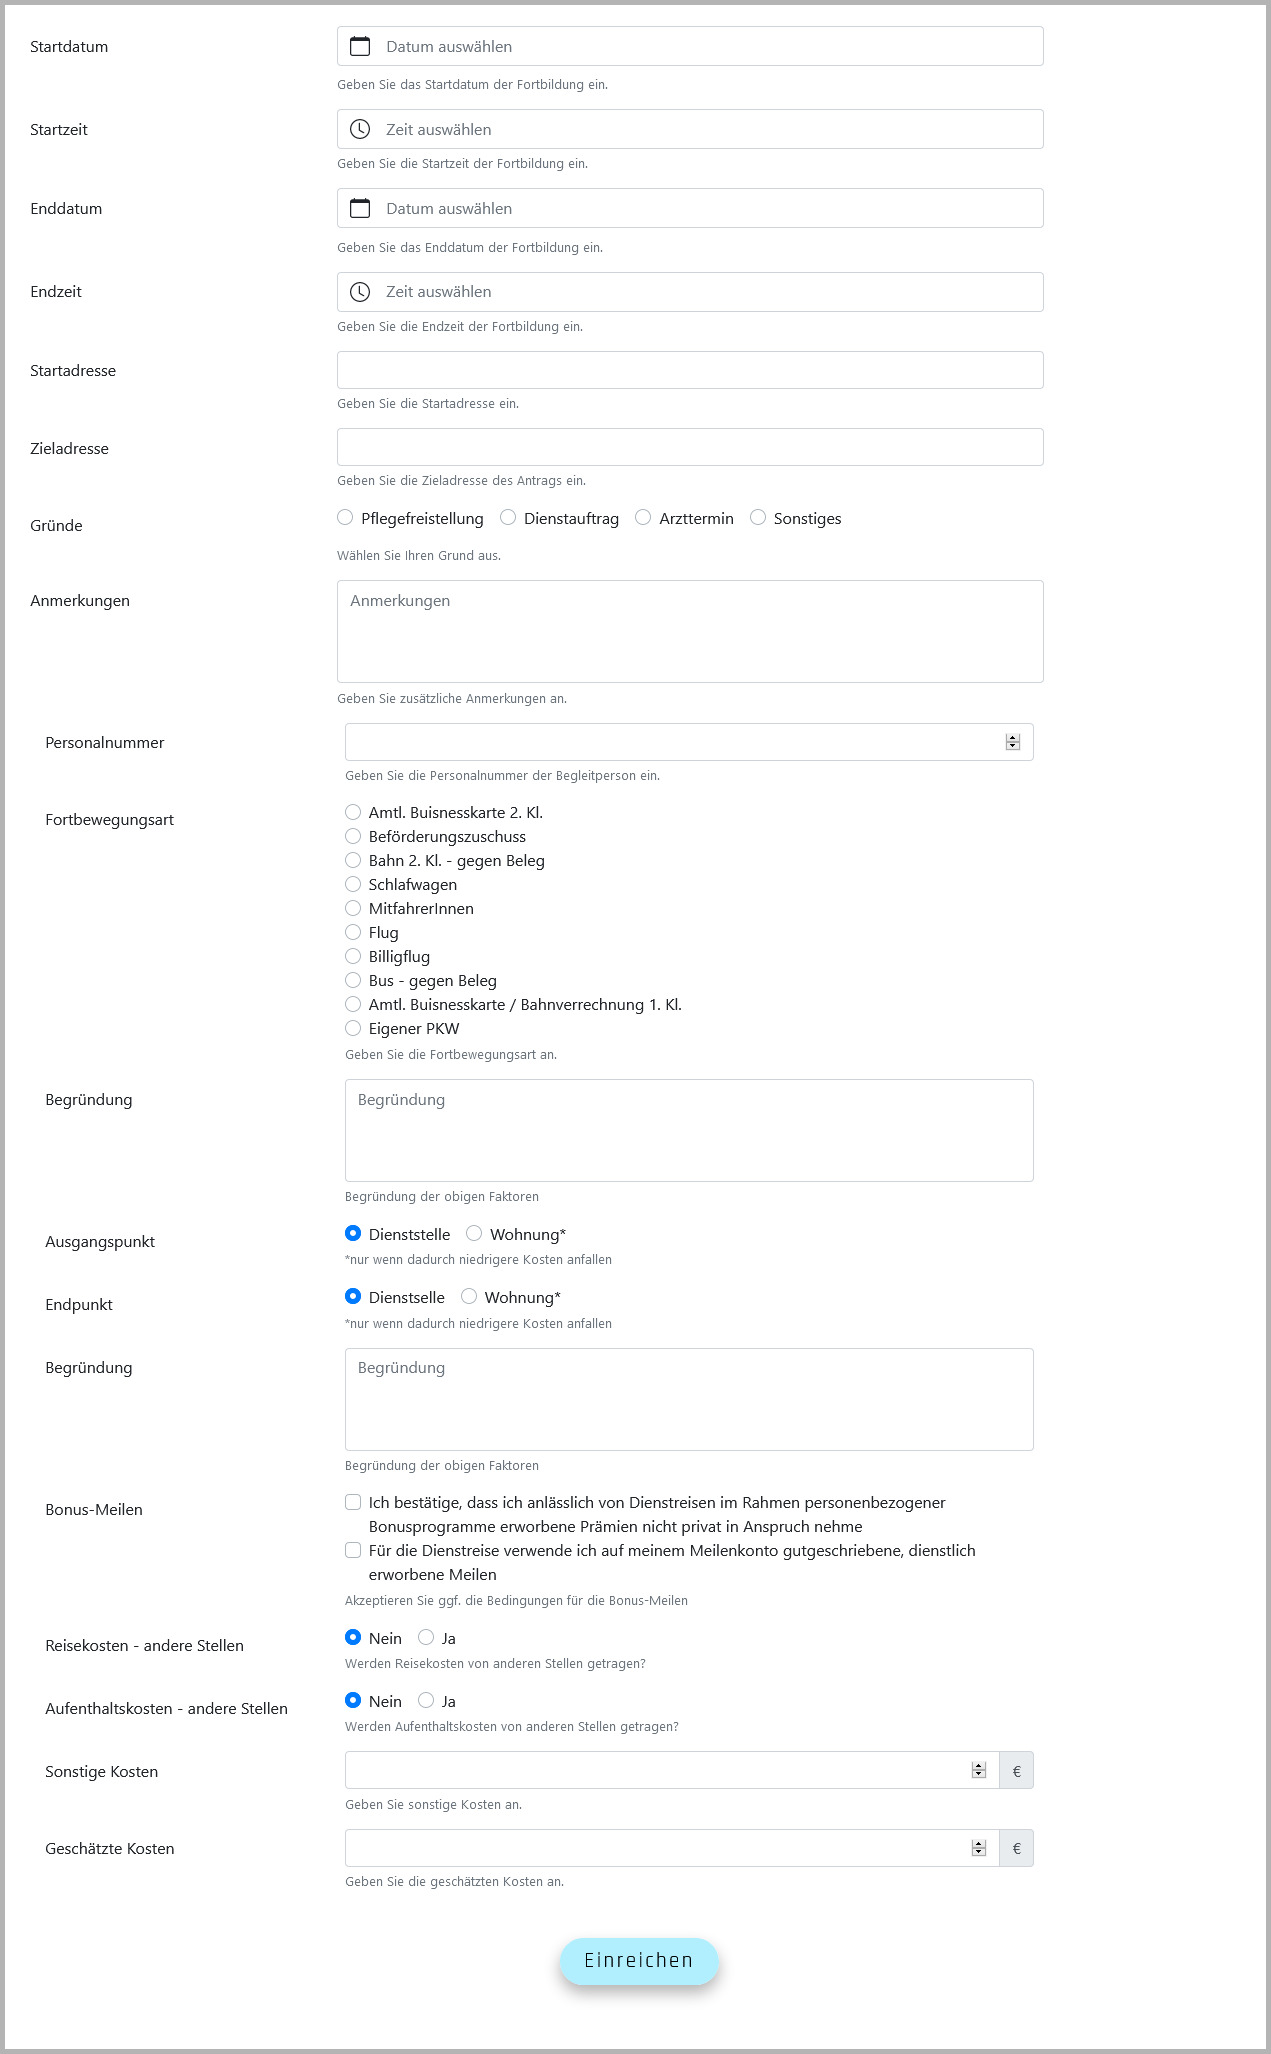
\includegraphics[width=0.75\linewidth]{images/othercause}
	\caption[Sonstiger Antrag]{Eingabefelder für sonstige Anträge}
	\label{fig:othercause}
\end{figure}
Sonstige Anträge werden unterschieden in Pflegefreistellungen, Dienstaufträgen, Arztterminen und Sonstiges. Das JSON-Objekt wird nach dem Drücken des ''Einreichen'' Knopfes erstellt und mit den angegebenen Daten befüllt. Das Objekt wird anschließend an das Backend gesendet.\\

Das JSON-Objekt wird, wie in Kapitel \hyperref[code_submit_data]{7.2.4.1} beschrieben, erstellt. Für einen Sonstigen Antrag gibt es nur wenige Änderungen.
Statt dem \textit{SchoolEventDetails} Objekt, wird ein \textit{OtherReasonDetails} Objekt in den Antrag hinzugefügt und die Art des Antrags wird auf 8 gesetzt:
\begin{code}{js}
var data = {		// Das JSON-Objekt mit allen Informationen
	Name: this.returnString(this.escorts.description),	// Der Name des Antrags
	Kind: 8,	// Der Typ des Antrags (8 = Sonstiger Antrag)
	// ...
	OtherReasonDetails: {
		Kind: this.returnValue(this.selected),	// Die Art des Sonstigen Antrags
		MiscellaneousReason: this.returnString(this.son),	// Falls "Sonstiges" ausgewählt worden ist
		ServiceMandateGZ: this.returnValue(this.gz),	// Die GZ des Dienstauftrags
		ServiceMandateTitle: this.returnString(this.title)	// Titel des Dienstauftrags
	},
	BusinessTripApplications: business,	// Das Reiseformular für den Lehrer
	TravelInvoices: invoices	// Die Reiserechnung für den Lehrer
};
\end{code}
\captionof{listing}{JSON-Objekt eines Sonstigen Antrags}~\\
\newpage
\subsection{Antrag Ansicht}
\label{sec:antrag_ansicht}
Wenn die Unterseite, die einen Antrag anzeigen soll, geladen wird, so wird der Unterseite die ID des Antrags mitgegeben. Mit dieser ID wird, sobald die Komponente geladen wird, eine Abfrage an das Backend gesendet, um den gesamten Antrag zu laden. Die Informationen werden interpretiert und angezeigt.
\subsubsection{Progress Bar}
Jeder Antrag besitzt einen Fortschritt, welcher graphisch durch eine \textit{Progress} Komponente angezeigt wird. Die Komponente erhält von der Antrag Ansicht den Fortschritt des Antrags und die Art des Antrags als Nummer, um die Informationen für den Benutzer lesbar anzuzeigen.
\begin{figure}
	\centering
	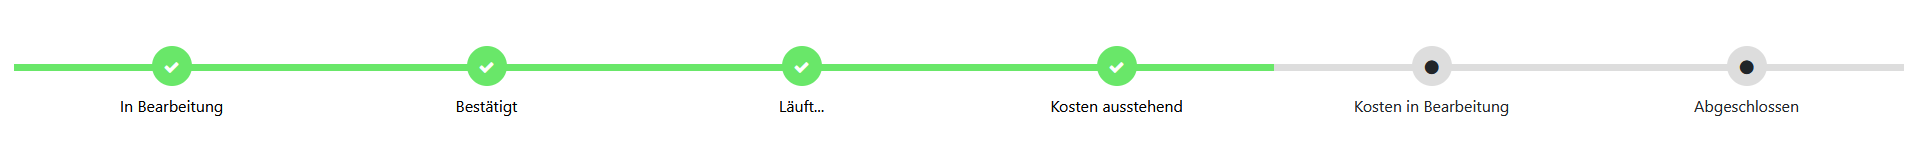
\includegraphics[width=1\linewidth]{images/progress}
	\caption[Fortschrittsanzeige]{Fortschrittsanzeige für einen Antrag}
	\label{fig:progress}
\end{figure}
\subsubsection{Dokumente}
In einem Antrag werden mehrere Dokumente gespeichert. Die Dokumente können je nach Fortschritt des Antrags bearbeitet werden.
Die Dokumente werden in einer Liste angezeigt:
\begin{figure}
	\centering
	
\includegraphics[width=1\linewidth]{images/documents}
	\caption[Dokumente eines Antrags]{Die Dokumente einer Schulveranstaltung}
	\label{fig:documents}
\end{figure}

Folgende Dokumente werden je nach Antragsart erstellt:
\paragraph{Schulveranstaltung}~\\
Die Schulveranstaltung besitzt zwei Dokumente. Zum Einen die allgemeinen Informationen zu der Veranstaltung und zum Anderen die Informationen zu den Begleitpersonen.
\subparagraph{Allgemeine Informationen}~\\
In diesem Dokument werden generellen Informationen über die Schulveranstaltung gespeichert. Diese können nur von dem Leiter des Antrags eingesehen und bearbeitet werden.
\subparagraph{Informationen zu Begleitlehrern}~\\
In diesem Dokument sieht jeder Begleitlehrer sein eigenes Formular, welches er je nach Fortschritt des Antrags bearbeiten kann. In diesem Dokument werden Informationen über die An-, Abreise und Aufenthalt des Lehrers gespeichert.
\paragraph{Fortbildung}~\\
In einem Fortbildungsformular werden Informationen über die Fortbildung und den Lehrer gespeichert.
\paragraph{Sonstiges}~\\
In einem ''Sonstiges'' Antrag werden Informationen über den Grund des Antrags, sowie den Zeitraum gespeichert.
\paragraph{Reiseformular}~\\
Ein Reiseformular wird bei jeder Art von Antrag erstellt. In einem Reiseformular werden Informationen über den Lehrer und über dessen An- und Abreise gespeichert.
\paragraph{Reiserechnung}~\\
Eine Reiserechnung wird bei jeder Art von Antrag erstellt. In einer Reiserechnung werden Informationen über die Kosten des Antrags gespeichert und wie diese entstanden sind. Des weiteren können Belege hochgeladen werden, um diese dem Antrag zu hinterlegen.
\subsubsection{Aktionen}
\paragraph{PDF öffnen}~\\
Der Benutzer kann die PDFs der Dokumente öffnen. Die PDFs werden in einem neuen Tab im Browser angezeigt.\\
Mit folgendem Code wird eine PDF erstellt und in einem neuen Tab geöffnet:\cite{sof_pdf}
\begin{code}{js}
	let pdfWindow = window.open("");
	var fileName = "PDF";
	pdfWindow.document.write(
	"<html<head><title>" +
	fileName +
	"</title><style>body{margin: 0px;}iframe{border-width: 0px;}</style></head>"
	);
	pdfWindow.document.write(
	"<body><embed width='100\%' height='100\%' src='data:application/pdf;base64, " +
	encodeURI(pdf) +
	"#toolbar=0\&navpanes=0\&scrollbar=0'></embed></body></html>"
	);
\end{code}
\paragraph{Änderungen speichern}~\\
Der Benutzer kann die Änderungen eines Antrags speichern. Dies kann in bestimmten Phasen eines Antrags geschehen. Die Änderungen werden, sobald auf den ''Änderungen Speichern'' Knopf gedrückt wird, an das Backend gesendet.
\paragraph{Antrag schließen}~\\
Der Leiter eines Antrags kann den Antrag schließen. Sobald der Antrag geschlossen ist, wird dieser im Backend gelöscht.
\newpage
\subsection{Antrag Übersicht}
\label{sec:antrag_uebersicht}
Um einen Überblick über die Anträge zu haben, gibt es zwei Übersichtsseiten, welche die Anträge auflisten. In den Auflistungen sieht man die groben Daten des Antrags und kann diese in der Antrag Ansicht öffnen. Sobald eine Übersichtsseite aufgerufen wird, werden die Anträge abgefragt und in der Liste angezeigt.
\begin{figure}[H]
	\centering
	
\includegraphics[width=1\linewidth]{images/liste_antrag}
	\caption[Liste der Anträge]{Auflistung von Anträgen auf der Übersichtsseite}
	\label{fig:listeantrag}
\end{figure}

\subsubsection{Alle Anträge}
Auf dieser Übersichtsseite werden alle Anträge angezeigt, die mit dem angemeldeten Benutzer zusammenhängen.
\subsubsection{Aktive Anträge}
In der Auflistung der aktiven Anträge, werden alle Anträge angezeigt, welche nicht abgeschlossen sind. Ist nur ein Antrag in der Liste der aktiven Anträge, so wird der Antrag sofort in der Antrag Ansicht geöffnet.
\subsubsection{Aktionen}
\paragraph{Schnelle Informationen}~\\
Wird auf den Knopf ''Schnelle Informationen'' gedrückt, öffnet sich ein Fenster, in dem die groben Informationen angezeigt werden.
\paragraph{Antrag Betrachten}~\\
Wird auf den Knopf ''Antrag Betrachten'' gedrückt, wird der Antrag in der Ansicht geöffnet.
\newpage
\subsection{Administrator}
\subsubsection{Antrag Ansicht}
Der Aufbau der Antrag Ansicht ähnelt dem aus dem Kapitel \hyperref[sec:antrag_ansicht]{7.2.5}.\\
Ein Administrator kann alle Informationen eines Antrags einsehen und diesen akzeptieren. Des Weiteren können alle PDFs des Antrags geöffnet werden. Der Antrag kann auch abgelehnt werden, wodurch der Fortschritt zurückgesetzt wird. Wenn der Antrag abgelehnt wird, kann ein Grund für das Ablehnen angegeben werden. Der Antragsteller kann daraufhin die Informationen des Antrags aktualisieren und damit den Antrag erneut einreichen, oder den Antrag schließen.
\subsubsection{Antrag Übersicht}
Die Übersichtsseite für Administratoren ähnelt dem Aufbau aus dem Kapitel \hyperref[sec:antrag_uebersicht]{7.2.6}.\\
Der Administrator sieht wer den Antrag gestellt hat und kann mehrere Anträge auswählen um diese in einer PDF anzuzeigen.
Des Weiteren kann auf den Knopf ''Antrag beachten'' gedrückt werden, wodurch der Administrator auf die Antrag Ansicht für Administratoren weitergeleitet wird.